\documentclass[notitlepage, twocolumn]{article}
\usepackage{fullpage}
\usepackage[affil-it]{authblk}
\usepackage{hyperref}
\usepackage{algpseudocode}
\usepackage[]{algorithmicx}
\usepackage{algorithm}
\usepackage{amsfonts}
\usepackage{amsmath}
\usepackage{amssymb}
\usepackage{graphicx}
\usepackage[backend=bibtex, style=numeric]{biblatex}
\usepackage{caption}
\usepackage{pdfpages}

\captionsetup[ruled]{labelsep=period}

\makeatletter
\@addtoreset{algorithm}{section}% algorithm counter resets every section
\makeatother

\renewcommand{\thealgorithm}{\thesection.\arabic{algorithm}}

\addbibresource{report.bib}

\def\ft{\mathcal{F}}
\algblockdefx[spawn]{Spawn}{EndSpawn}
[1]{\textbf{spawn process for} #1 \textbf{do}}
{\textbf{end spawn}}

\def\CC{\mathbb{C}}	% Complex

\newcommand{\set}[1]{\lbrace #1 \rbrace}
\newcommand{\paren}[1]{\left( #1 \right)}

\title{\bf
GPU Accelerated Fast Fourier Transform
}

\date{December 2015}
\author{
Matt McCarthy
}
\affil{Christopher Newport University\\
\textbf{CPSC 621 Parallel Processing}\\
\texttt{\href{mailto:matthew.mccarthy.12@cnu.edu}{matthew.mccarthy.12@cnu.edu}}
}

\begin{document}
\nocite{*}
\maketitle

\noindent\textbf{Abstract}
We empirically investigate the performance benefits of parallel fast Fourier transform running on the GPU over a sequential version running on the GPU.

\section{Background}

\subsection{Discrete Fourier Transform}

The discrete Fourier transform is a mathematical transformation that takes a set of Complex-valued signals and outputs a set of Complex-valued frequencies.
For an $n$-dimensional Complex-valued vector $\mathbf{X}$, the discrete Fourier transform $\mathbf{Y}=\mathcal{F}(X)$ is given by
\[
	Y_j = \sum_{k=0}^n x_k \omega^{jk}
\]
where $\omega$ is the $n$-th root of unity, $e^{2\pi i/n}$.
Since $\mathbf{Y}$ is an $n$-dimensional, Complex-valued vector, we can see that the discrete Fourier transform has a complexity of $\Theta(n^2)$.

\subsection{Fast Fourier Transform}

Furthermore, we can split the discrete Fourier transform into even and odd sums for $n=2m$, yielding
\[
	Y_j = \sum_{k=0}^m x_{2k}\omega^{2jk} + \omega^j\sum_{k=0}^m x_{2k+1}\omega^{2jk}
\]
which is two separate discrete Fourier transforms.
Suppose $n=2^k$.
If we iterate this process, we get the following algorithm called the one-dimensional, unordered radix 2, fast Fourier transform in Algorithm 1.1.
\begin{algorithm}
	\caption{Recursive FFT}
	\begin{algorithmic}[1]
		\Function{R-FFT}{$\mathbf{X}$,$\mathbf{Y}$,$n$,$\omega$}
			\If{$n$=1}
				\State $y_0=x_0$
			\Else
				\State Let $\mathbf{Q}=\mathbf{0},\mathbf{T}=\mathbf{0}\in\CC^n$
				\State Let $\mathbf{X_e}=(x_0, x_2,\ldots,x_{n-2})$
				\State Let $\mathbf{X_o}=(x_1, x_3,\ldots,x_{n-1})$
				\State \Call{R-FFT}{$\mathbf{X_e}$,$\mathbf{Q_e}$,$n/2$,$\omega^2$}
				\State \Call{R-FFT}{$\mathbf{X_o}$,$\mathbf{T_o}$,$n/2$,$\omega^2$}
				\ForAll{$j\in\set{0,1,\ldots,n-1}$}
					\State $y_j=q_{j\mod{n/2}}+\omega^i t_{j\mod{n/2}}$
				\EndFor
			\EndIf
		\EndFunction
	\end{algorithmic}
\end{algorithm}

\subsubsection{Cooley Tukey}

Furthermore, we have an iterative formulation of the prior algorithm, called the Cooley Tukey algorithm for one-dimensional, unordered radix 2, fast Fourier transforms.

\begin{algorithm}
	\caption{Cooley-Tukey FFT}
	\begin{algorithmic}[1]
		\Function{I-FFT}{$\mathbf{X}$,$\mathbf{Y}$,$n$}
			\State $t:=\lg n$
			\State $\mathbf{R}=\mathbf{X}$
			\For{$m=0$ to $t-1$}
				\State $\mathbf{S}=\mathbf{R}$
				\For{$l=0$ to $n-1$}
					\State Let $(b_0b_1\ldots b_{t-1})$ be the binary expansion of $l$
					\State $j:=(b_0\ldots b_{m-1}0b_{m+1}\ldots b_{t-1})$
					\State $k:=(b_0\ldots b_{m-1}1b_{m+1}\ldots b_{t-1})$
					\State $r_i:= s_j+s_k\omega^{(b_mb_{m-1}\ldots b_0 0\ldots0)}$
				\EndFor
			\EndFor
			\State $\mathbf{Y}:=\mathbf{R}$
		\EndFunction
	\end{algorithmic}
\end{algorithm}

From this pseudo-code, we can determine the complexity of fast Fourier transform as described by Algorithm 1.2.
We begin by noting that we iterate through the outer loop precisely $\lg n$ times and the inner loop $n$ times.
Therefore our complexity is $T_1=\Theta(n\lg n)$.

\subsection{Parallelization}

For our parallelization, we use a simplified version of the binary exchange algorithm, a parallelization of the Cooley Tukey algorithm designed for use on a hypercube.
Since our implementation runs on a single GPU, any thread can access any memory location via a pointer.
However, this also complicates the matter by introducing a potential for data races.
We solve this by modifying the algorithm to work as follows in Algorithm 1.3.
\begin{algorithm}
	\caption{Parallel FFT}
	\begin{algorithmic}[1]
		\Function{PAR-FFT}{$\mathbf{X}$,$\mathbf{Y}$,$n$}
			\State $t:=\lg n$, $BLK:=n/p$
			\State $\mathbf{R}=\mathbf{X}$
			\State $\mathbf{S}=\mathbf{0}$
			\For{$m=0$ to $t-1$}
				\State Swap pointers $\mathbf{R}$ and $\mathbf{S}$
				\Spawn{$l=0$ to $BLK-1$}
					\For{$c=l\cdot BLK$, to $l\cdot(BLK+1)$}
						\State Let $(b_0b_1\ldots b_{t-1})$ be the binary expansion of $c$
						\State $j:=(b_0\ldots b_{m-1}0b_{m+1}\ldots b_{t-1})$
						\State $k:=(b_0\ldots b_{m-1}1b_{m+1}\ldots b_{t-1})$
						\State $r_i:= s_j+s_k\omega^{(b_mb_{m-1}\ldots b_0 0\ldots0)}$
					\EndFor
				\EndSpawn
				\State \textbf{sync}
			\EndFor
			\State $\mathbf{Y}:=\mathbf{R}$
		\EndFunction
	\end{algorithmic}
\end{algorithm}
In each iteration, we only write to $\mathbf{R}$ and only read from $\mathbf{S}$.
Since we wait until each thread is complete before moving on to the next iteration, we avoid the potential to use old or incorrect data.

If we inspect the parallelization, we see that the outer loop runs $\lg n$ times.
However, the inner loop is ran on $p$ processes, each of which handle $n/p$ iterations.
Therefore, the computation cost is $\Theta(n/p\lg n)$.
Moreover, for communication we simply do two reads from VRAM on each iteration of the inner loop, however some values will be in cache so we may get better performance than that.
Ergo, the communication cost is $O(n/p\lg n)$.
Thus, the parallel runtime will be $T_p = \Theta(n/p \lg n)$ and is cost optimal if and only if $p\leq n$.

\section{Experimental Design}

The goal of the experiment is to empirically determine the effect of parallelization on the runtime of the Cooley Tukey algorithm.
To this end we want to measure the runtime of fast Fourier transform using differing sizes of $n$, the dimension of our Complex valued vector, and $t$, the number of threads.
Let $\mathcal{N}$ be the set of vector dimensions we will test and let $\mathcal{T}$ be the set of thread counts we will test.
Furthermore, we specify that each $n\in\mathcal{N}$ and each $t\in\mathcal{T}$ be powers of two.

For $t=1$, we will run the Cooley Tukey algorithm on random Complex valued vectors of dimension $n$ for each $n\in\mathcal{N}$.
Otherwise, we run our parallelization of the Cooley Tukey algorithm on Complex valued vectors of dimension $n$ for each $n\in\mathcal{N}$.
Moreover, before and after each run, we copy the input to the GPU and the output from the GPU.
We take the system time before copying the input to the GPU and again after copying the output to the host.
We do not check the output for correctness during the test in order to save time, but instead checked the correctness of the algorithm beforehand.

\section{Test Environment}

\subsection{Test System}

The machine used to run the test has an Intel i7 4770k running at 4.2GHz, 16GB of RAM, and a Nvidia GTX 970 with a core clock of 1342MHz and memory clock of 7000MHz.
The computer was running Arch Linux on Linux kernel 4.2.5 with Nvidia driver version 358.16 and CUDA 7.5.

\subsection{Test Program}

Firstly, all code can be located at \url{https://github.com/matt-mccarthy/fast-fourier-transform} in the \verb|fast-fourier| folder.
We also include a version of the code in the Appendix.

We wrote all code in CUDA C++.
Furthermore all code was compiled with the CUDA toolkit 7.5 and GCC 5.2.0 using the command \verb|nvcc| \verb| -std=c++11| \verb|-rdc=true| \verb|-arch=compute_52| \verb|-code=sm_52 -O3|.
The library source file is \verb|src/fast-fourier.cu|, and the sequential and parallel main functions are located in \verb|sequential-fft.cu| and \verb|parallel-fft.cu| respectively.

In both the sequential fast Fourier and parallel fast Fourier, we ran into issues with dynamically allocating memory in a CUDA kernel.
Namely, if we allocated and freed often enough, we ran out of memory.
To avoid this issue entirely, we made all allocations of giant arrays occur in main once and then reused those arrays.
As a note, the \verb|binary_stor| array is where we store the binary representation of our index $l$ for each thread.
While this design is suboptimal (ideally, each thread would create its own so others can not touch it), it works and the performance impact should be neglible for large enough $n$.

Moreover, our GPU code is entirely without any conditional statements except the ones for determining whether or not our for loop is within its bounds.
Another note about the code is that at the end of each iteration of the outer for loop, we call \verb|cudaDeviceSynchronize| which blocks until our \verb|transformer| kernel completes.
We do this in order to ensure syncrhonization across all threads and prevent data races.
Furthermore, the \verb|transformer| kernel must always be called from another kernel that runs on exactly one thread.
We do this in order to keep all code running on the device and prevent useless communication between the CPU and GPU.

For our test we took, $\mathcal{N}=\set{2^{17},2^{19},2^{21},2^{23},2^{25}}$ and $\mathcal{T}=\set{1,4,16,64,256,1024}$, all of which are less than the number of cores on our GTX 970.
We chose $\mathcal{N}$ such that we would get a runtime for 1MB of data on the low end, and 1GB of data on the high end since each complex value is a typedef'd \verb|float2|.
Moreover, we ran each combination of $n$ and $t$ 10 times each.
All runtimes were measured and recorded in milliseconds, and our result files are included in Appendix B.

\section{Results}

\begin{figure}\label{results}
	\centering

	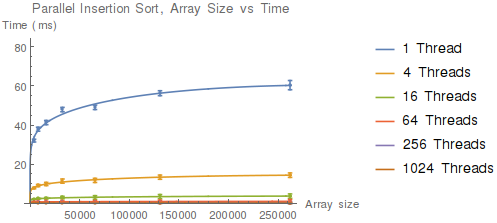
\includegraphics[scale=0.35]{results.png}
	\caption{Runtime vs Array Size}
\end{figure}

\begin{figure}\label{res-table}
	\centering
	\begin{small}
	\[
		\begin{array}{r|c|c|c|c|c}
			& 2^{17} & 2^{19} & 2^{21} & 2^{23} & 2^{25}\\\hline
			2^0& 7.37 & 35.8 & 162 & 773 & 3.42\cdot10^6\\\hline
			2^2& 1.75 & 8.47 & 38.5 & 183  & 813\\\hline
			2^4& .446 & 2.15 & 9.75 & 46.4 & 205.8\\\hline
			2^6& .117 & .552 & 2.51 & 11.9 & 52.8\\\hline
			2^8& .034 & .149 & .669 & 3.14 & 14.3\\\hline
			2^{10}& 0.011 & .046 & .201 & .975 & 4.65
		\end{array}
	\]
	\end{small}
	\caption{The table of runtimes at $(n,t)$ in s}
\end{figure}

Figure 2 lists the runtimes for each $t$ (row index) at size $n$ (column index).
Moreover, the graphs all look like the standard $x\ln x$ curve.
By inspection, we see that $T_{2k}\approx T_{2k+2}/4$, which is exactly what we are looking for.
So naively, we can say that this has a linear speedup.

We also attempted to compute on 1GB of random complex numbers, or precisely, $2^{27}$ complex numbers.
The parallel runtime for $t=1024$ was approximately 22s, however, after many hours of running the sequential version at this $n$ did not complete.
Upon deeper analysis, we learned that with perfect linear speedup, the sequential version would have a runtime roughly 1000 times greater than $T_{1024}$, namely 6 hours.
Due to time constraints, we had to abandon this size of $n$ and make our maximum $2^{25}$.
Furthermore, due to memory constraints, we could not test for any $n\geq 2^{28}$ since we have to allocate two arrays of 2GB each in order to compute on it and our 970 has 4GB VRAM.

\section{Future Work}

In our study, VRAM limitations and time constraints prevented us from harnessing extremely large values of $n$.
One way to extend this study to larger values of $n$ is to simply use GPUs that have more than 4GB of VRAM like the Titan X and simply run tests with larger values of $n$.

Another, more interesting path to explore is to distribute the problem across multiple GPUs.
If we split it smartly, we should be able to utilize the extra VRAM without incurring too much communication overhead.
Of course, the inter-GPU communication is also a factor and we would need to decide the best way to manage it.
This latter method can also scale to a GPU farm.

\section{Conclusion}

Our analysis of the algorithm determined that for $t \leq n$, we should get perfect linear speedup and the data provides empirical evidence for that, with 1024 threads executing approximately 1000 times faster than the sequential.

\printbibliography

\end{document}
